\documentclass[11pt]{ctexart}

\usepackage{multicol}
%\usepackage{mwe}
\usepackage{subfigure}
\usepackage{mathtools}
\usepackage{graphicx}
\usepackage{amsmath}
\usepackage{mathrsfs}
\usepackage[top=0.5in,bottom=1in,left=1in,right=1in]{geometry}
\usepackage{pdflscape}
\usepackage{times}
\usepackage{bm}
%\usepackage{setspace}
\usepackage{color}
\usepackage{caption}
\usepackage{amsmath}
\usepackage{amssymb}
\usepackage{CJK}
\usepackage{longtable}
%\usepackage[final]{pdfpages}
\usepackage{listings}
\usepackage{textcomp}
\usepackage{xcolor}
\usepackage{algorithm2e}
\usepackage{float}
\usepackage{algorithmicx}
\usepackage{algpseudocode}
\usepackage{hyperref}

\hypersetup{hidelinks,
	colorlinks=true,
	allcolors=black,
	pdfstartview=Fit,
	breaklinks=true}

\pagestyle{plain}




\begin{document}

\title{第九周实习报告20220520}
\author{宋欣源}
\date{\today}

\maketitle % need full-width title

\CTEXsetup[format={\Large\bfseries}]{section}

\section{第一,综述}

下面对于这些天实习的工作做一个报告。现在就两周的工作做一个总结
我这周主要在raw3数据集上进行。首先将过去的cnn1d,cnn2d,rnn,convrnn,transformer模型进行全部的调试和运行,然后从这些方向里选择cnn1d的新模型一直继续研究。

\section{第二,CNN2d}
\subsection{1.模型和表现}

模型1:普通CNN2d(ordinary*2+pointwise+linear*2+dropout+relu)

{\kaishu \small IC: 0.059, pnl:2.2}

~\\
模型2:普通CNN2d(deepwise*2+pointwise+linear*2+dropout+relu)

{\kaishu \small IC: 0.059, pnl:2.3}


~\\
模型3:普通CNN2d(ordinary*2+linear*2+pointwise+linear*2+dropout+relu)

{\kaishu \small IC: 0.068, pnl:2.47}


~\\
模型4:普通CNN2d(deepwise*2+linear*2+pointwise+linear*2+dropout+relu)

{\kaishu \small IC: 0.062, pnl:2.52}


~\\
模型5:普通CNN2d(deepwise*2+maxpool+linear*2+pointwise+linear*2+dropout+relu)

{\kaishu \small IC: 0.062, pnl:2.4}


~\\
模型6:普通CNN2d(deepwise*2+ordinary+linear*2+pointwise+linear*2+dropout+relu)

{\kaishu \small IC: 0.066, pnl:2.2}


~\\
模型7:普通CNN2d(deepwise*2+ordinary*3+linear*2+pointwise+linear*2+dropout+relu)

{\kaishu \small IC: 0.068, pnl:2.4}


~\\
整体来看,在raw3数据上表现强于raw5数据,但是raw5数据拥有时间尺度的变化,raw3数据变化有限,raw5数据最高做到2.5的情况,raw3很容易地达到了结果。基础表现也比较强。

\subsection{2.改进思路}
\begin{itemize}
  \item [0)]
  对原来的模型框架进行了整个修改和重置。我觉得在这些在CNN2d模型上能取得的效果已经尽可能发掘了。单纯从CNN提取信息的角度感觉很难发掘出新的东西。下面一部就是开发新的模型,采取新的思路,单纯增加模型的深度已经满足不了要求了,模型会在第四个epoche上开始效果下降,具有过拟合的风险。而且对于CNN2d本身来说,从模型上控制过拟合的办法,比如resnet,dialtion,增加感受野之类的办法,在32*12的数据上很难使用。因此后面不再继续深入CNN2d的研究。
\end{itemize}

\begin{figure}[H]
\begin{center}
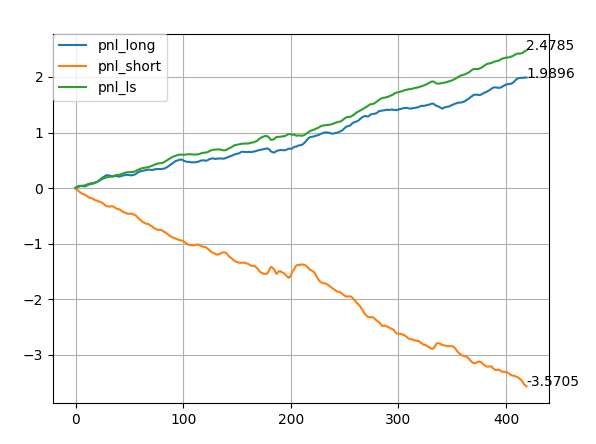
\includegraphics[width=0.8\textwidth]{plt1.PNG}
\end{center}
\caption{modelCNN2d pnl figure}
\label{FIG.1}
\end{figure}

\section{第三,CNN1d}
\subsection{1.模型和表现}

模型8:普通CNN1d(ordinary*2+avg+linear*2+dropout+relu)

{\kaishu \small IC: 0.053, pnl:2.2}


~\\
模型9:普通CNN1d(ordinary*2+avg+ordinary*2+linear*2+dropout+relu)

{\kaishu \small IC: 0.055, pnl:2.3}


~\\
模型10:普通CNN1d(ordinary*2+avg+ordinary*2+linear*2+pointwise+dropout+relu)

{\kaishu \small IC: 0.054, pnl:2.4}


~\\
模型11:普通CNN1d((ordinary+avg+relu)*3+ordinary+linear*2+dropout+relu)

{\kaishu \small IC: 0.052, pnl:2.3}



~\\
模型12:普通CNN1d((ordinary+avg+relu)*4+ordinary+pointwise+linear*2+dropout+relu)

{\kaishu \small IC: 0.056, pnl:2.3}


~\\
模型13:普通CNN1d((ordinary+avg+relu)*5+ordinary+pointwise+linear*2+dropout+relu)

{\kaishu \small IC: 0.057, pnl:2.3}


~\\
模型14:普通CNN1d((ordinary+avg+relu)*6+ordinary+pointwise+linear*2+dropout+relu)

{\kaishu \small IC: 0.061, pnl:2.35}


~\\
模型15:普通CNN1d((ordinary+avg+relu)*7+ordinary+pointwise+linear*2+dropout+relu)

{\kaishu \small IC: 0.060, pnl:2.24}

模型深度已经很深,不便于继续加深,在largeFOV的backbone下已经不适合继续深入。继续深入模型表现已经没有提升。总体来看,largeFOV的backbone不适合CNN1d在模型上的深入,下面是bottleneck的backbone进行深入。原来的思路是deeplab在时间序列上的特征提取,现在由于数据减少,原来模型的深度减少进行进一步探索。

~\\
模型16:bottleneck((cnn1d(1)+cnn1d(3)+cnn1d(1))+pointwise+linear+dropout+relu)

{\kaishu \small IC: 0.061, pnl:2.4}

关于bottleneck的backbone进行简单叙述:bottleneck方法主要用来训练CNN神经网络,可以降低数据维度,先用bottleneck层作为人为升高数据的隐藏维度,在高维数据中提取信息,因为信息损失,就会减少高频噪声,就可以提取较好的特征,再用bottleneck层人为降低维度,再次进行模型简化,很大的避免了过拟合,算法如下:
\renewcommand{\algorithmicrequire}{\textbf{Input:}}  % Use Input in the format of Algorithm
\renewcommand{\algorithmicensure}{\textbf{Output:}} % Use Output in the format of Algorithm
  \begin{algorithm}[htb]
  \caption{bottleneck structure}
  \label{alg:Framwork}
  \begin{algorithmic}[1]
    \Require
      1 channel 42 * 280000 time series dataloader;
      3*3 线性卷积核;
      5*5 线性卷积核;
    \Ensure
      1 channel 277200 return 或者277200其他高维特征;
    \State 升维convolution(input:1 channel, output:100 channel,kernelsize: 1);
    \label{code:fram:extract}
    \State 维度转换convolution(input:100 channel, output:100 channel,kernelsize: 5);
    \label{code:fram:trainbase}
    \State 特征提取convolution(input:100 channel, output:100 channel,kernelsize: 3);
    \label{code:fram:trainbase}
    \State batchnorm2d;
    \label{code:fram:trainbase}
    \State relu(0.1);
    \label{code:fram:select}
    \State 降维convolution(input:100 channel, output:50 channel,kernelsize: 1);
    \label{code:fram:decrease}
    \State 残差层shortcut;
    \label{code:fram:residual}
    \State 特征提取convolution(input:100 channel, output:50 channel,kernelsize: 3);
    \label{code:fram:residual}
    \State batchnorm2d;
    \label{code:fram:residual}
    \State relu(0.5);
    \label{code:fram:residual}

    \Return residual bottleneck+ residual shortcut;
  \end{algorithmic}
\end{algorithm}

~\\
模型17:bottleneck((cnn1d(1)+cnn1d(3)+cnn1d(1))+pointwise+linear+dropout+relu)


{\kaishu \small IC: 0.062, pnl:2.4}

可以看出bottleneck的结构更适合raw3数据。


~\\
模型18:base((cnn1d+batchnorm+relu+avgpool)*2+pointwise+linear+dropout+relu)

消融实验:对largeFOV的结构加入batchnorm,效果变化不大

{\kaishu \small IC: 0.061, pnl:2.2}


~\\
模型19: bottleneck((cnn1d+batchnorm+relu+avgpool)*2+bottleneck1+pointwise

+linear+dropout+relu)

加入bottleneck的backbone以后模型解读能力提高。

{\kaishu \small IC: 0.065, pnl:2.5}



~\\
模型20: bottleneck((cnn1d+batchnorm+relu+avgpool)*2+bottleneck2+pointwise

+linear+dropout+relu)

对于压缩和提升维度的bottleneck2,和第一种效果区别不大

{\kaishu \small IC: 0.063, pnl:2.52}



~\\
模型21: bottleneck((cnn1d+batchnorm+relu+avgpool)*2+bottleneck1+bottleneck2+pointwise

+linear+dropout+relu)

bottleneck1和bottleneck2一起并行,效果有小量提升

{\kaishu \small IC: 0.065, pnl:2.58}



~\\
模型22: deeplab((cnn1d+batchnorm+relu+avgpool)*2+bottleneck1

+bottleneck2+bottleneck1+bottleneck2+pointwise+linear+dropout+relu)

{\kaishu \small IC: 0.068, pnl:2.62}

\begin{figure}[H]
\begin{center}
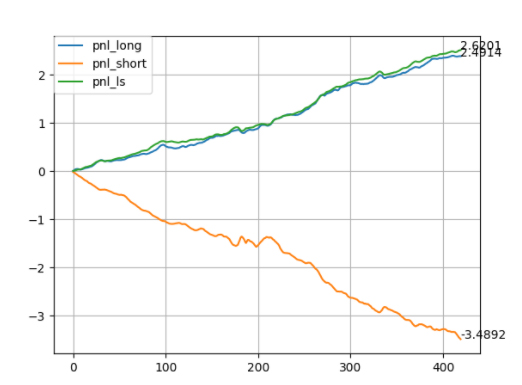
\includegraphics[width=0.8\textwidth]{plt2.PNG}
\end{center}
\caption{model\_deeplab pnl figure}
\label{FIG.2}
\end{figure}


~\\
模型23: multibox(base+multibox+poitwise)

下面对于上次研究的multibox目标检测网络进行复现,原来的网络需要的序列较长,因此进行修改。

multibox系列网络,IC比较高,但是pnl表现一般

{\kaishu \small IC: 0.073, pnl:2.2}

当模型复杂的时候,序列越短模型表现越不稳定,长序列的优点是模型稳定,短序列则表现不太稳定,往往需要多次run才能得到理想的结果。原因很容易解释,长序列中进行目标检测更容易检测到特定的pattern,而对于短序列更容易错误检测

~\\
模型24: multibox+bottleneck(base+bottleneck+multibox+linear)

将bottleneck和multibox进行合并,提高了IC同时提高了pnl

{\kaishu \small IC: 0.071, pnl:2.58}

\begin{figure}[H]
\begin{center}
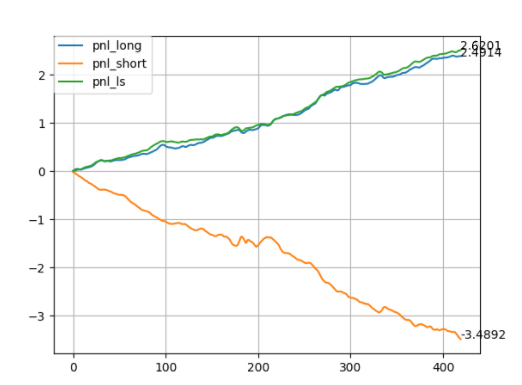
\includegraphics[width=0.8\textwidth]{plt3.PNG}
\end{center}
\caption{model\_bottleneck+multibox pnl figure}
\label{FIG.2}
\end{figure}

~\\
模型25:multibox+bottleneck

继续深入

{\kaishu \small IC: 0.072, pnl:2.3}


~\\26:multibox+bottleneck+pointwise+linear+relu

计算出的结果还是一样。

{\kaishu \small IC: 0.067, pnl:2.3}


~\\

模型27:multibox+bottleneck+downsample

对于bottleneck+multibox应用了downsample,好处是可以将数据进行归纳,减少高维数据直接接fc的情况,对于时间序列提取信息更友好。从信息流的角度,将高维特征进行降维,得到更有意义的特征,无意义的特征都会被downsample降低为0,和maxpool加matrix形式一样。

{\kaishu \small IC: 0.064, pnl:2.47}


~\\
模型28:multibox+downsample

对于bottleneck做消融实验

{\kaishu \small IC: 0.070, pnl:2.2}


~\\
模型29:multibox++downsample+upsample

对downsample重新upsample,另一种消融方式

{\kaishu \small IC: 0.065, pnl:2.5}


~\\
模型31:multibox+multibox+downsample+upsample

将两个multibox进行叠加,在没有bottleneck的backnbone的情况下效果有提升

{\kaishu \small IC: 0.068, pnl:2.58}


\subsection{2.改进思路}
\begin{itemize}
  \item [0)]
  在bottleneck的情况下,可以改进bottleneck的结构,比如原来研究的bottleneck3,bottleneck4的结构,进行替换研究。
  \item [1)]
  在multibox上还有很多改进的地方,比如下面要研究的FCOS网络,是multibox的新的backbone.目前消融实验表明,multibox对于普通deepnn,bottleneck都有提高,所以可以进一步提高。
  \item [2)]
  在deeplab领域,已经不适合现在的任务,模型backbone已经不再适用于新的任务,以后不再对deeplabV3进行研究。
\end{itemize}


\section{第四、RNN的研究:convolutedRNNcell}
\subsection{综述}
这次主要是重新run了convolutedRNN的结果,比raw5数据更好,还有深入的空间。对RNNcell和RNN主体backbone模型还要再raw3上进行实验。目前模型待跑。


\subsubsection{convGRU}

模型1:convGRU(conv+linear)\_2layer(layer1(batch:1,kernel:3), layer2(batch:1,kernel:3)) 

{\kaishu \small IC: 0.037, pnl:2.0}

~\\
模型2:convGRU(conv+linear)\_2layer(layer1(batch:n,kernel:1), layer2(batch:n,kernel:1)) 

{\kaishu \small IC: 0.042, pnl:2.2}

~\\
模型3:convGRU(conv+linear)\_2layer(layer1(batch:n,kernel:1), layer2(batch:1,kernel:3)) 

{\kaishu \small IC: 0.049, pnl:2.2}


~\\
模型4:convGRU(conv+conv)\_2layer(layer1(batch:1,kernel:3), layer2(batch:1,kernel:3)) 

{\kaishu \small IC: 0.050, pnl:2.3}

~\\
模型5:convGRU(conv+conv)\_2layer(layer1(batch:n,kernel:1), layer2(batch:n,kernel:1)) 

{\kaishu \small IC: 0.048, pnl:2.2}

~\\
模型6:convGRU(conv+conv)\_2layer(layer1(batch:n,kernel:1), layer2(batch:1,kernel:3)) 

{\kaishu \small IC: 0.053, pnl:2.2}


~\\
模型7:convGRU(linear+conv)\_2layer(layer1(batch:1,kernel:3), layer2(batch:1,kernel:3)) 
{\kaishu \small IC: 0.052, pnl:2.4}

~\\
模型8:convGRU(linear+conv)\_2layer(layer1(batch:n,kernel:1), layer2(batch:n,kernel:1)) 

{\kaishu \small IC: 0.051, pnl:2.3}

~\\
模型9:convGRU(linear+conv)\_2layer(layer1(batch:n,kernel:1), layer2(batch:1,kernel:3)) 

{\kaishu \small IC: 0.050, pnl:2.4}

~\\
模型10:convGRU(conv+conv)\_4layer(layer1(batch:n,kernel:1), layer2(batch:n,kernel:1), layer3(batch:1, kernel:3),layer4(batch:1, kernel:3)) 

{\kaishu \small IC: 0.059, pnl:2.6}


\subsubsection{convLSTM等其他模型}
LSTM,convLSTMC,conv\_passcell\_1,conv\_passcell\_2
关于这几类模型,还要修改数据输入和输出,目前还没有跑完。


\section{第六、总结}
\begin{itemize}
  \item [1)]
  第一,CNN2d系列模型,经过大量模型设计和修正,单纯从提取信息的角度,已经挖掘到了瓶颈。CNN2d不适合raw3任务。
  \item [2)]
  第二,对于convolutedRNN模型,以及原来设计的RNN的backbone我不打算深入研究,打算把之前的模型在raw3上进行复现,挑选不错的模型进行收集。
  \item [3)]
  第三,对于CNN1d系列,已经尝试了bottleneck,multibox,deeplab三种backbone(对于resnet50,VGG这类模型深度太高,不适合尝试),下一步目标明确,就是在multibox的基础上实验FCOS网络,并且和目前已知的几种表现良好的模型做组合和消融实验。
\end{itemize}


\end{document} 